% Chapter 4

\chapter{CA Guide Mobile Application} % Main chapter title

\label{frontend} % For referencing the chapter elsewhere, use \ref{Chapter1} 

\lhead{Chapter 4. \emph{Museum Guide Frontend}} % This is for the header on each page - perhaps a shortened title

%----------------------------------------------------------------------------------------

\section{Target Platform}

The target mobile plattform for the CA Guide frontend application is iOS 8.1. The targeted mobile device is an iPad mini with GPS sensor. This device was choosen for it's compact size and light weight, while still offering much more screen size than a normal smartphone, which is advantageous for displaying images and text in a size that is more comfortable to read.

\section{Architecture}

The application is separated in 5 different layers.

%TODO Figure without data
\begin{figure}[H]
\centering
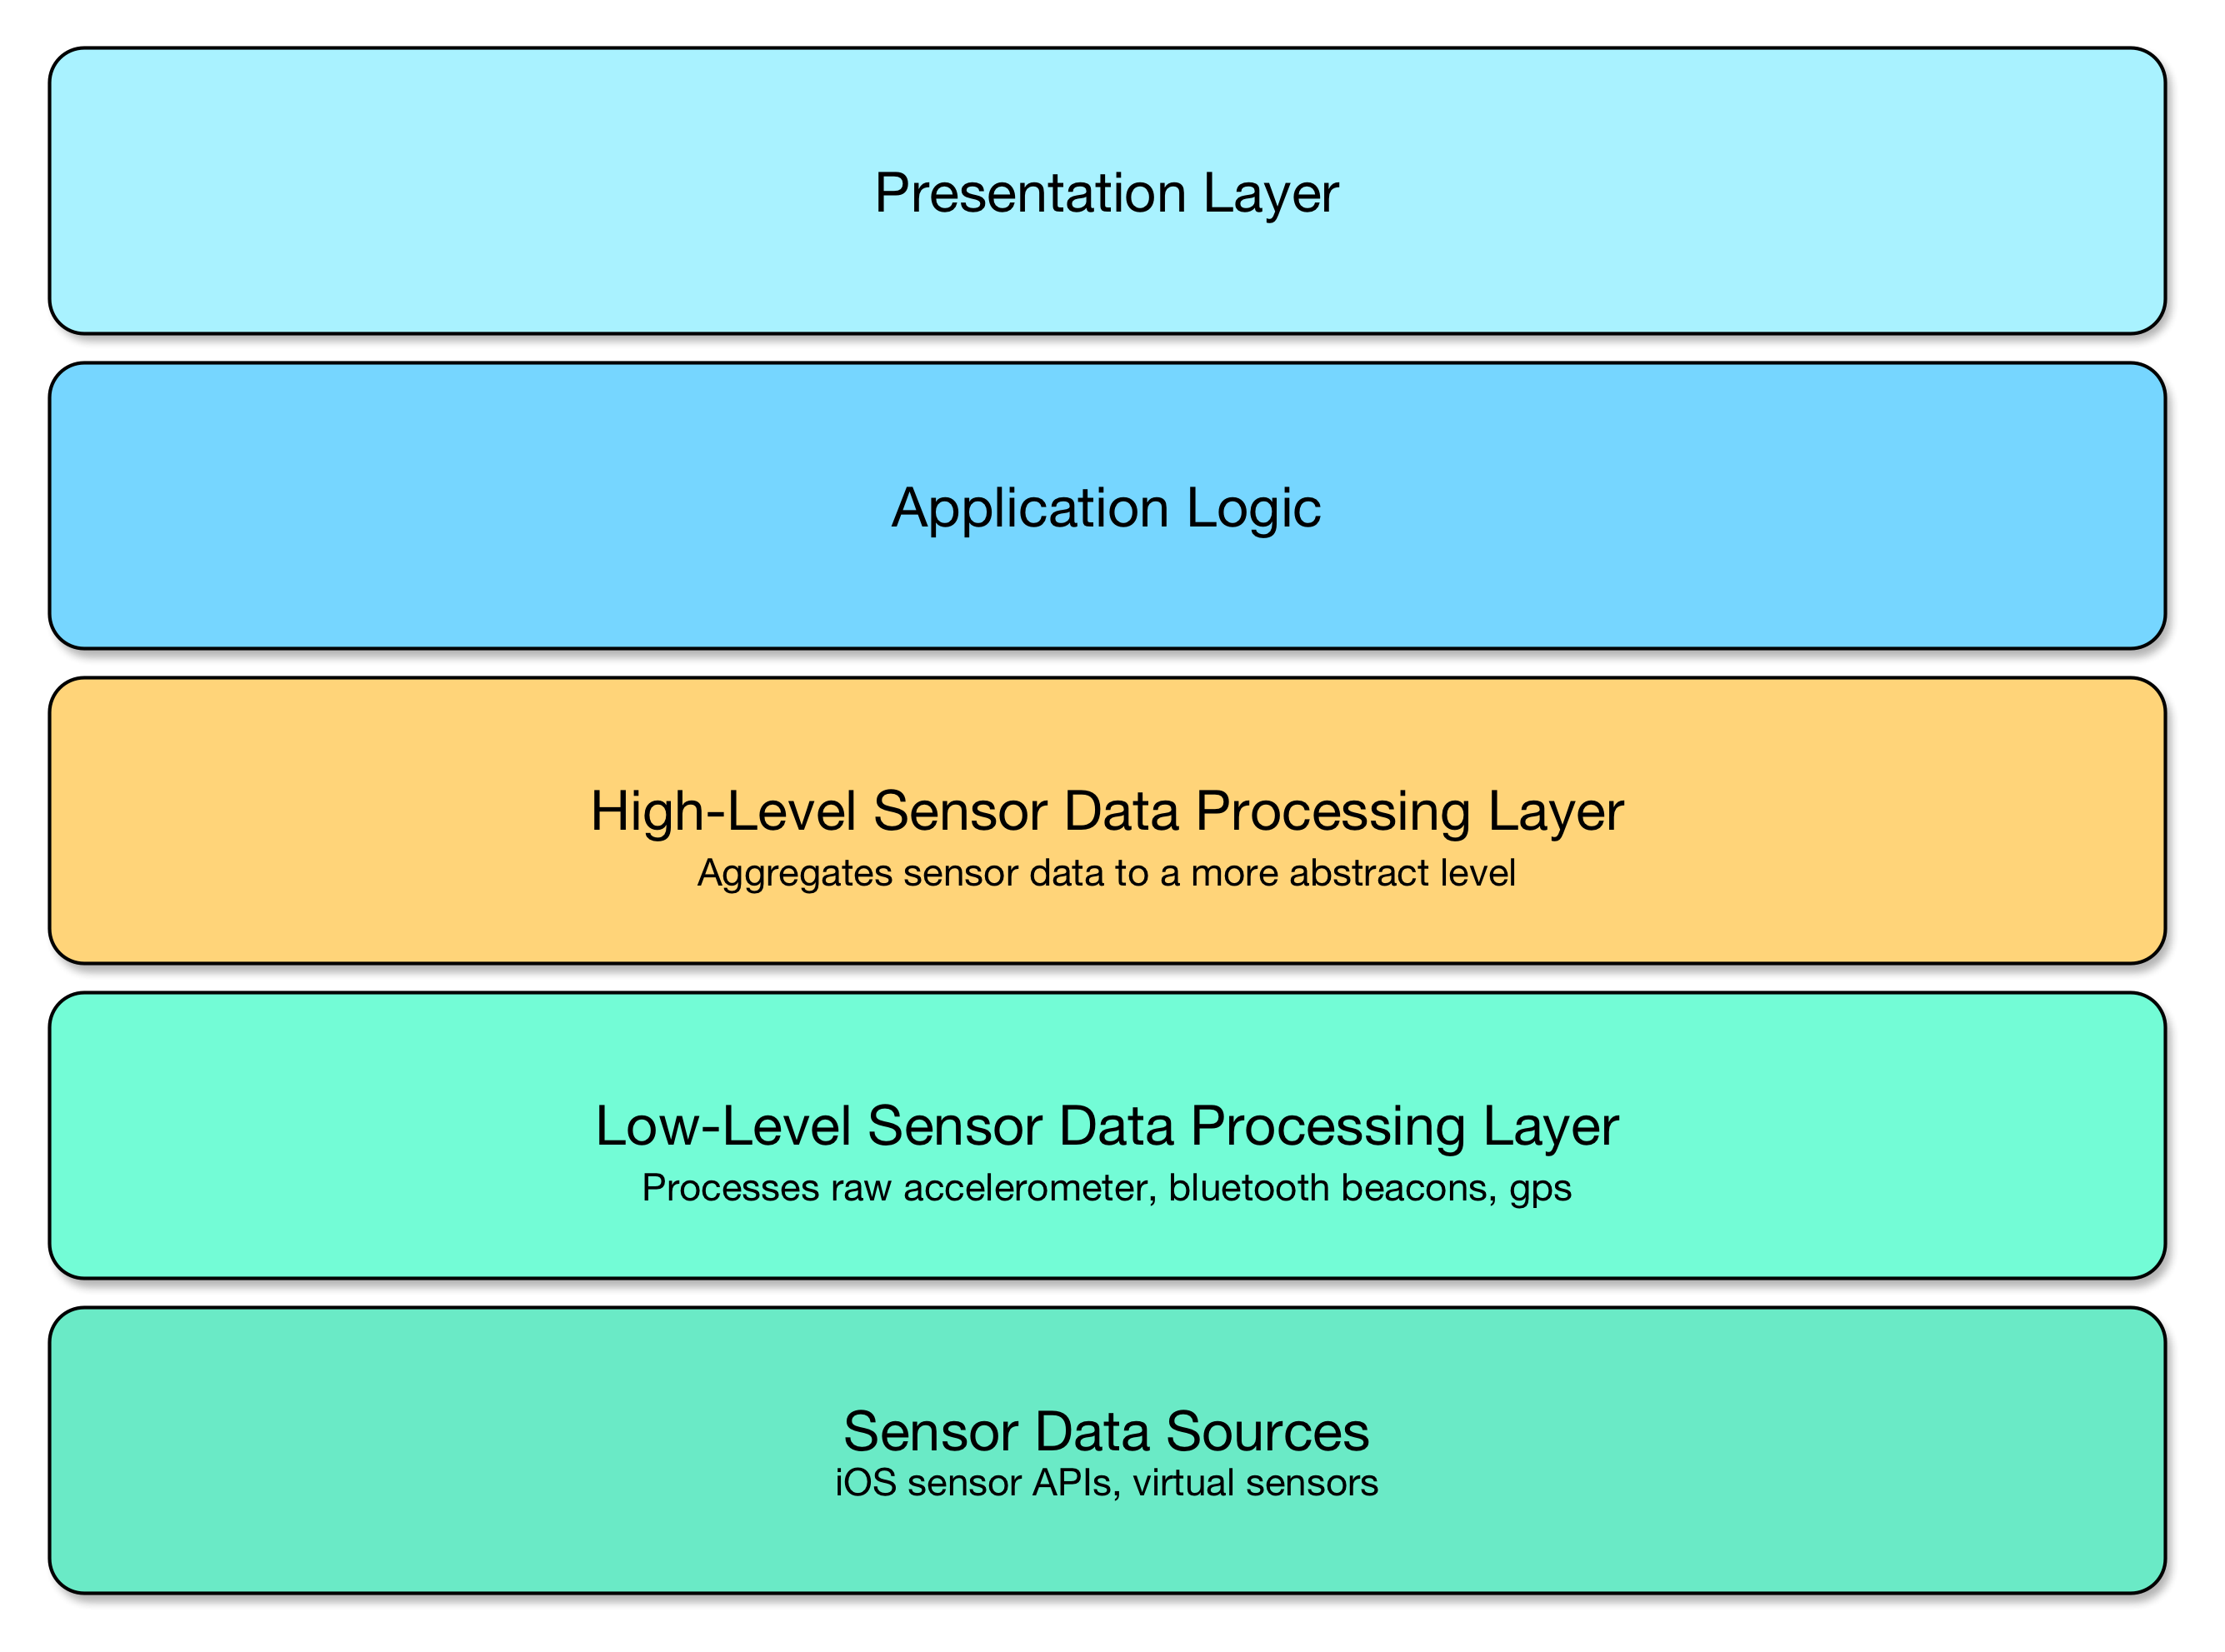
\includegraphics[width=0.9\textwidth]{layers-guide-app.png}
\caption{Layer Model of the Museum Guide Application}
\end{figure}

A fundamental requirement for the CA Guide frontend, the mobile application, is the ability to automatically test the single layers using recorded sensor data and comparing it with it's expected result.

To achieve this level of testability, virtual sensors are introduced at three different levels of abstraction:
 
\begin{figure}[H]
\centering
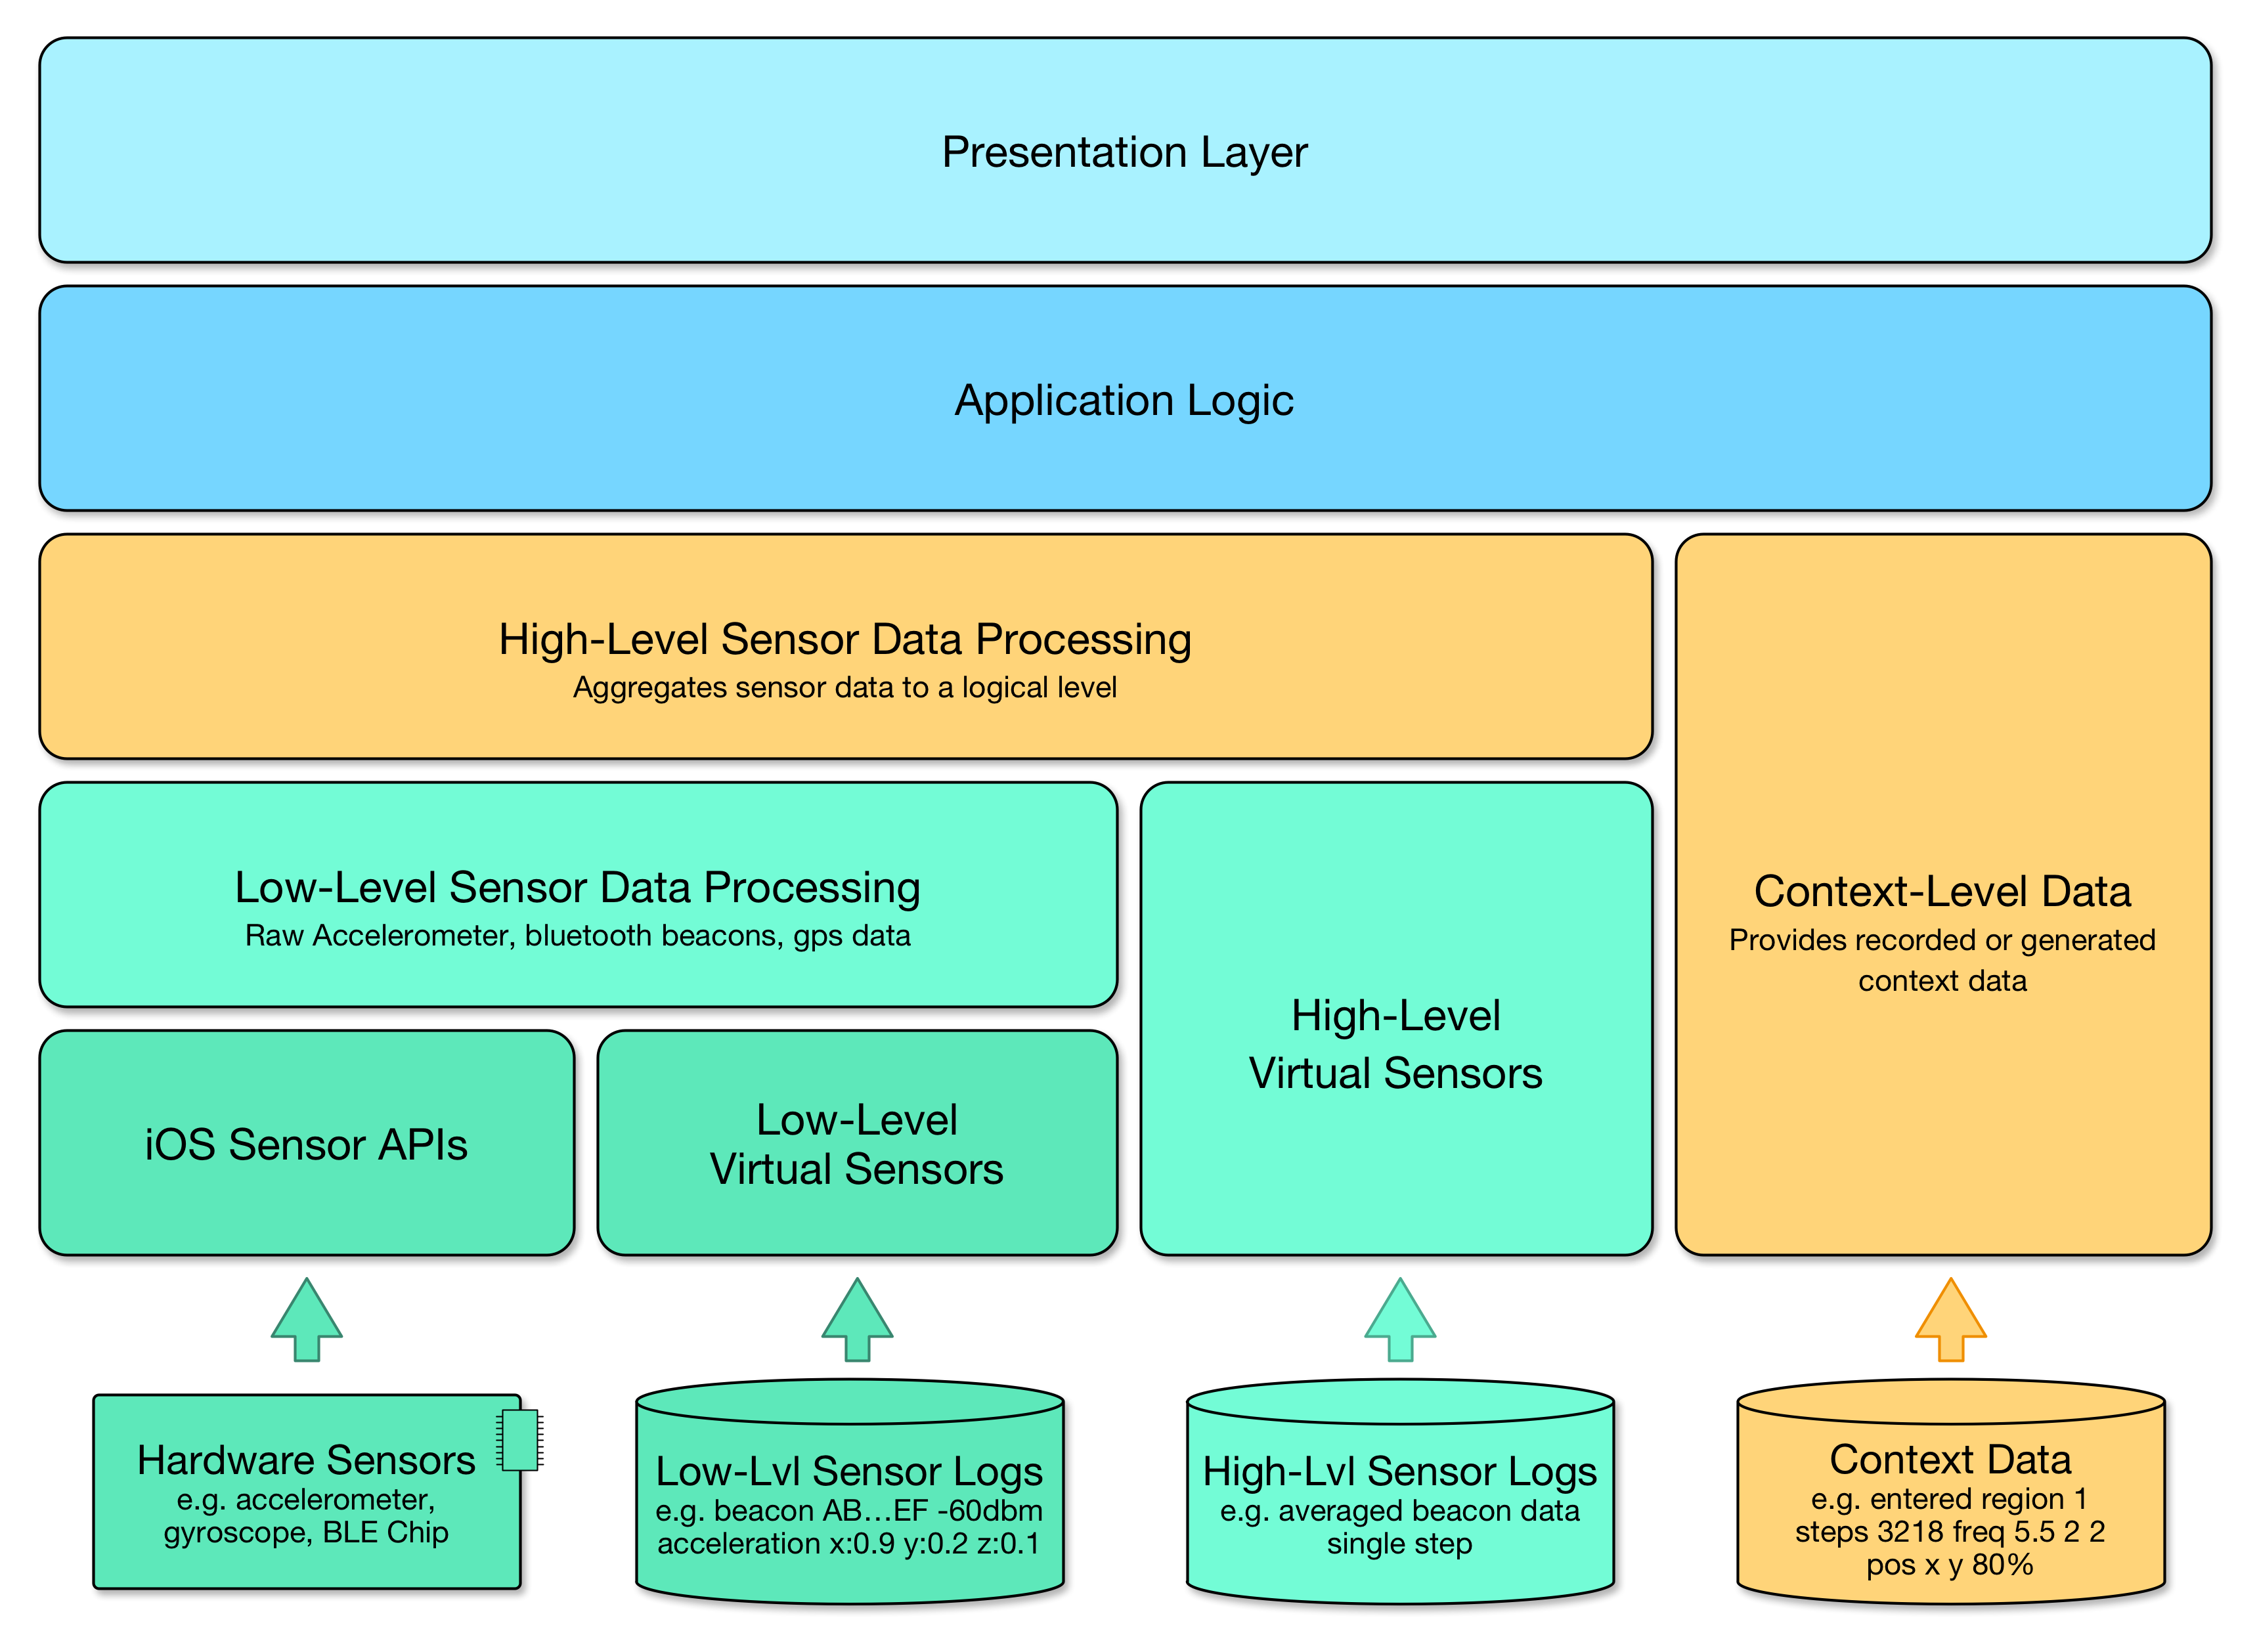
\includegraphics[width=0.9\textwidth]{layers-guide-refined-app.png}
\caption{Layer Model with virtual sensors}
\end{figure}

The following figure visualizes the different kind of data that is handled in every different layer, taking the accelerometer data processed by pedometer and statistics algorithms as an example. The frequency of events passed to the next layer decreases from real-time data (100 updates per second), demanding very fast algorithms, to some seconds or minutes.

\begin{figure}[H]
\centering
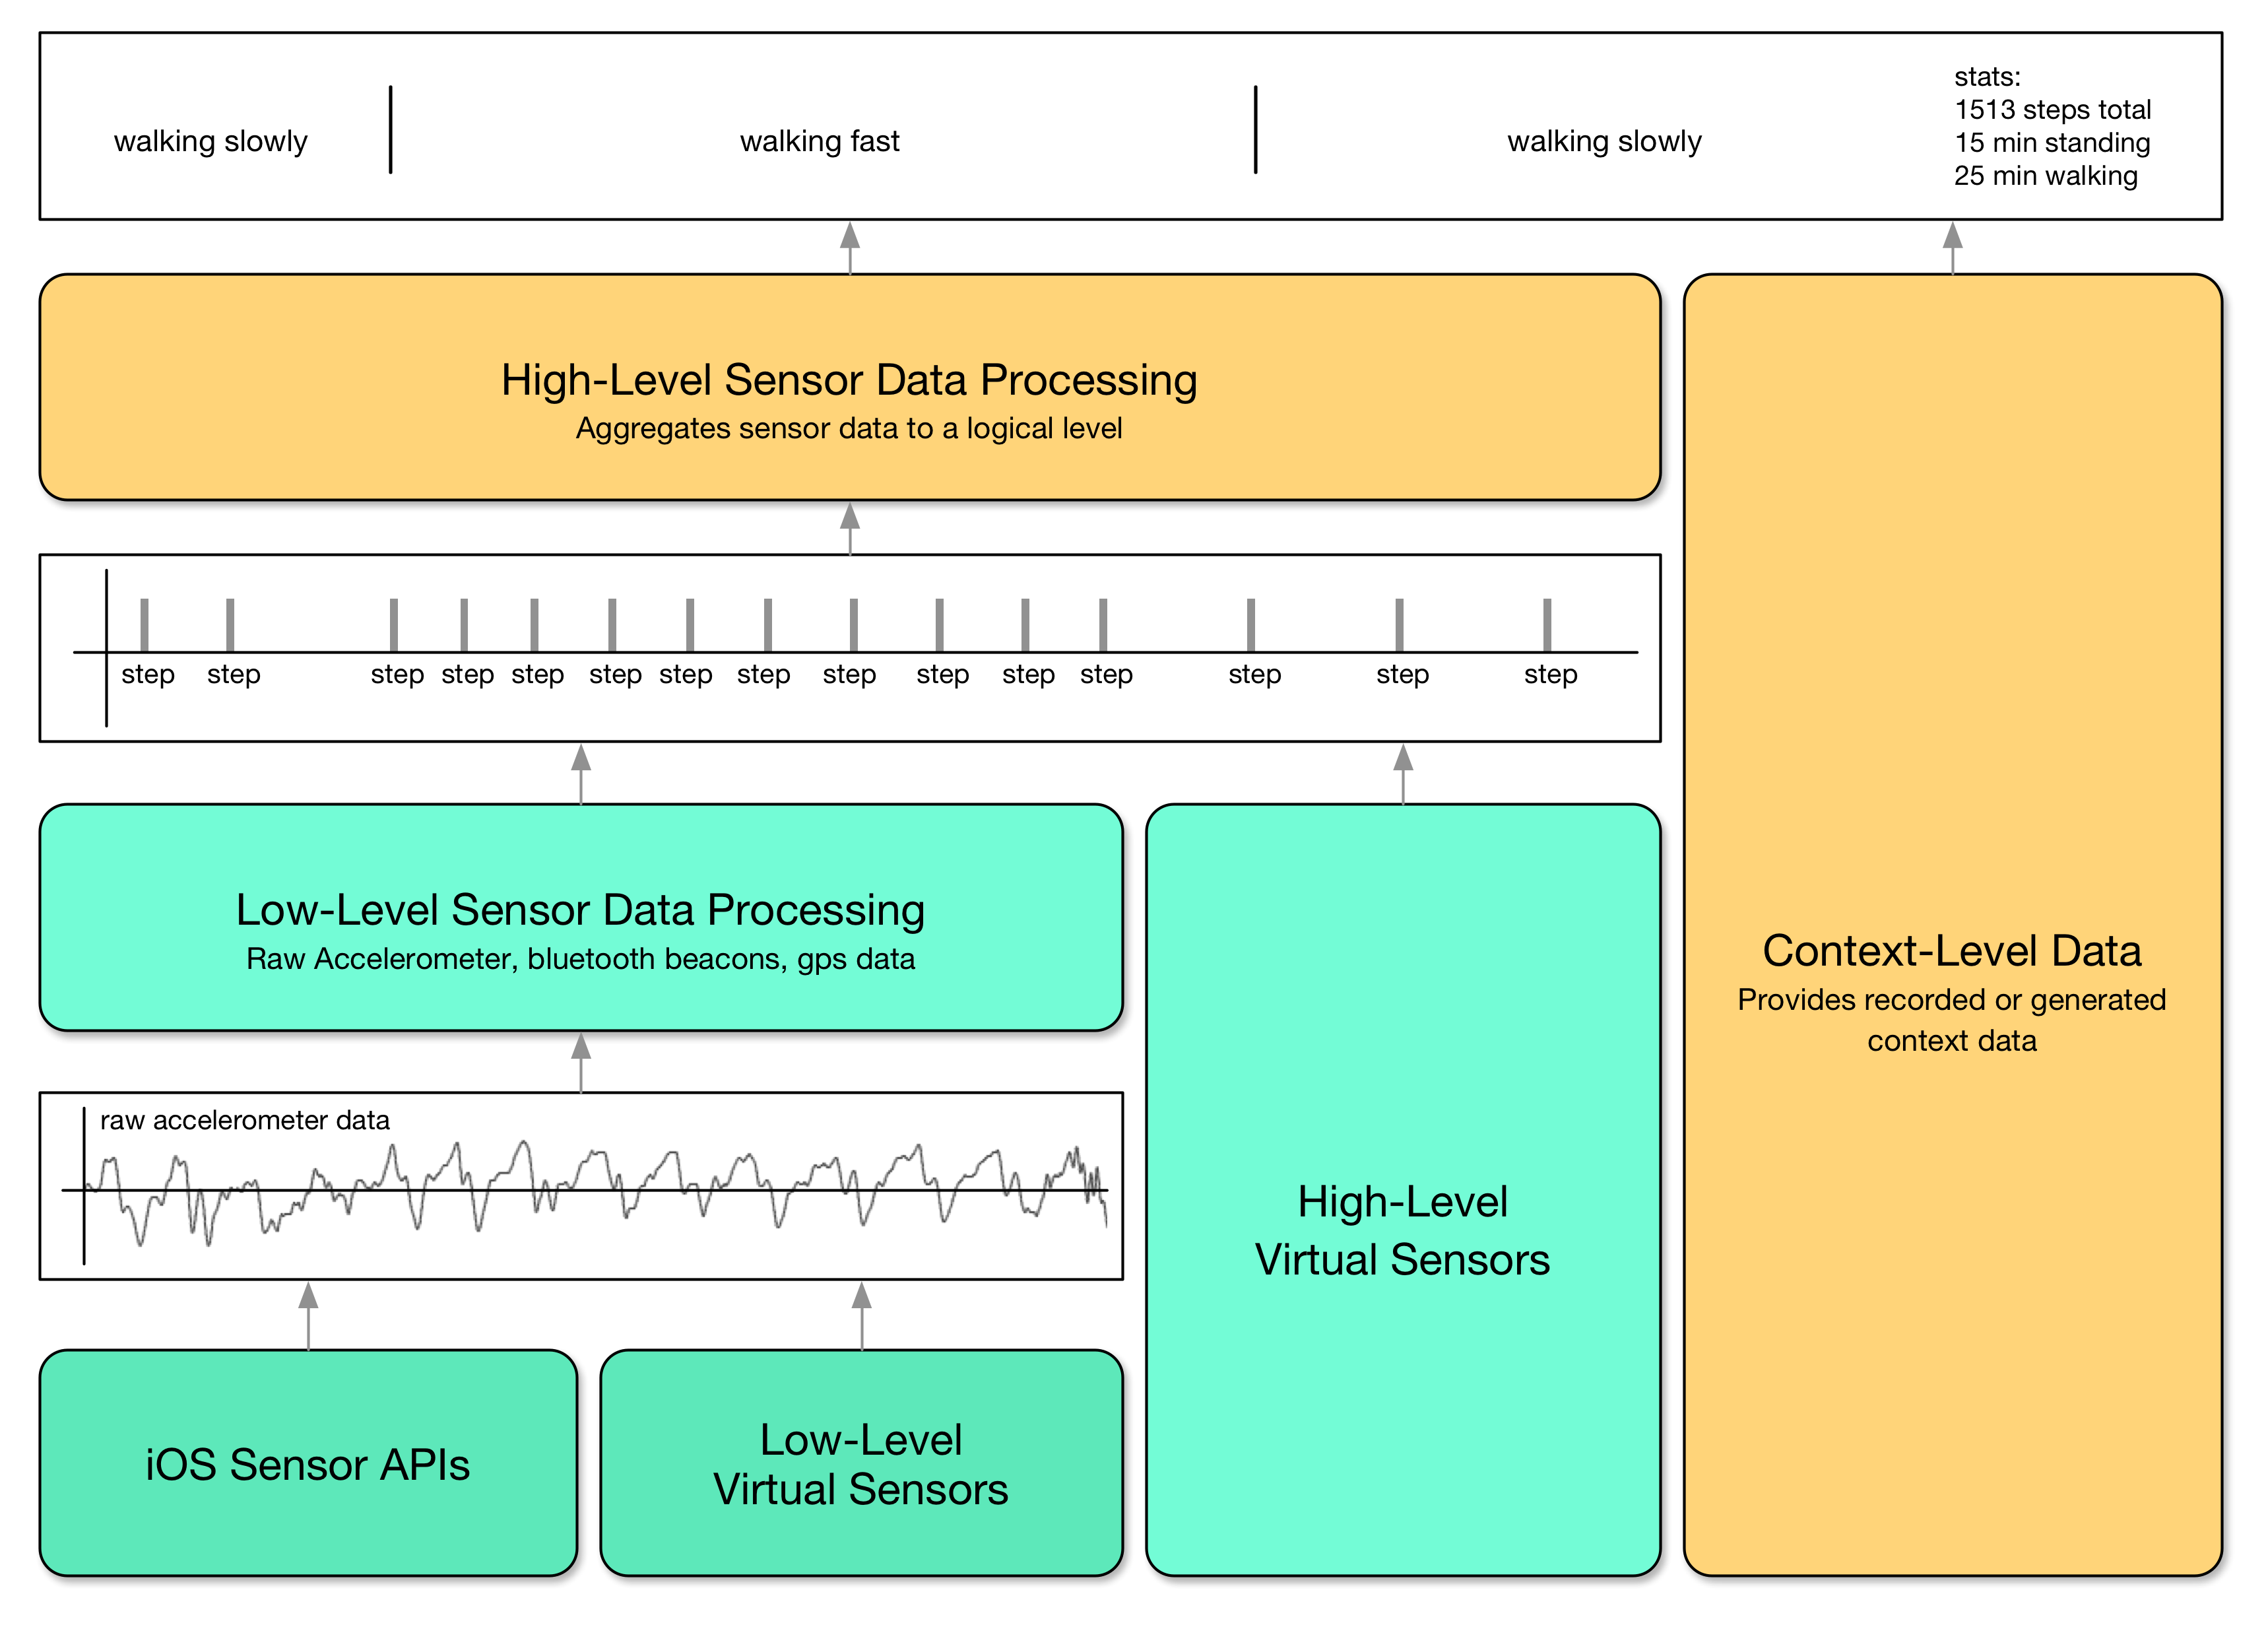
\includegraphics[width=0.9\textwidth]{layers-app-dataflow-accelerometer.png}
\caption{Data Flow between the lower Layers}
\end{figure}

The pedometer algorithm in the low-level sensor data processing layer receives raw accelerometer data as input. It analyzes the data, detects single steps and passes them to the upper layer, the high-level sensor data processing. Here the single steps are aggregated to periods of slow and fast walking and walking statistics are updated.

Beside enabling automated unit tests at different abstraction levels, this layered virtual sensor concept has various other benefits:

\begin{itemize}
\item During development, a simulation of walking through a park or museum is possible, for manually testing not only algorithms of the lower layers, but also elements of the uppermost layer like different screen transitions or other UI behavior.
\item For demonstration the guide to customers or prospects a walk through a park can be simulated at the desk on a real device running the guide, beeing much more intuitive than showing only screen shots.
\item With an own class in the Sensor APIs layer acting as an adapter to the iOS APIs it is easier to migrate the algorithms to a different mobile platform, by rewriting this adapter class for the target platforms Sensor API and automatically translating the other sources that have no dependencies to the platform.
\end{itemize}



\begin{figure}[H]
\centering
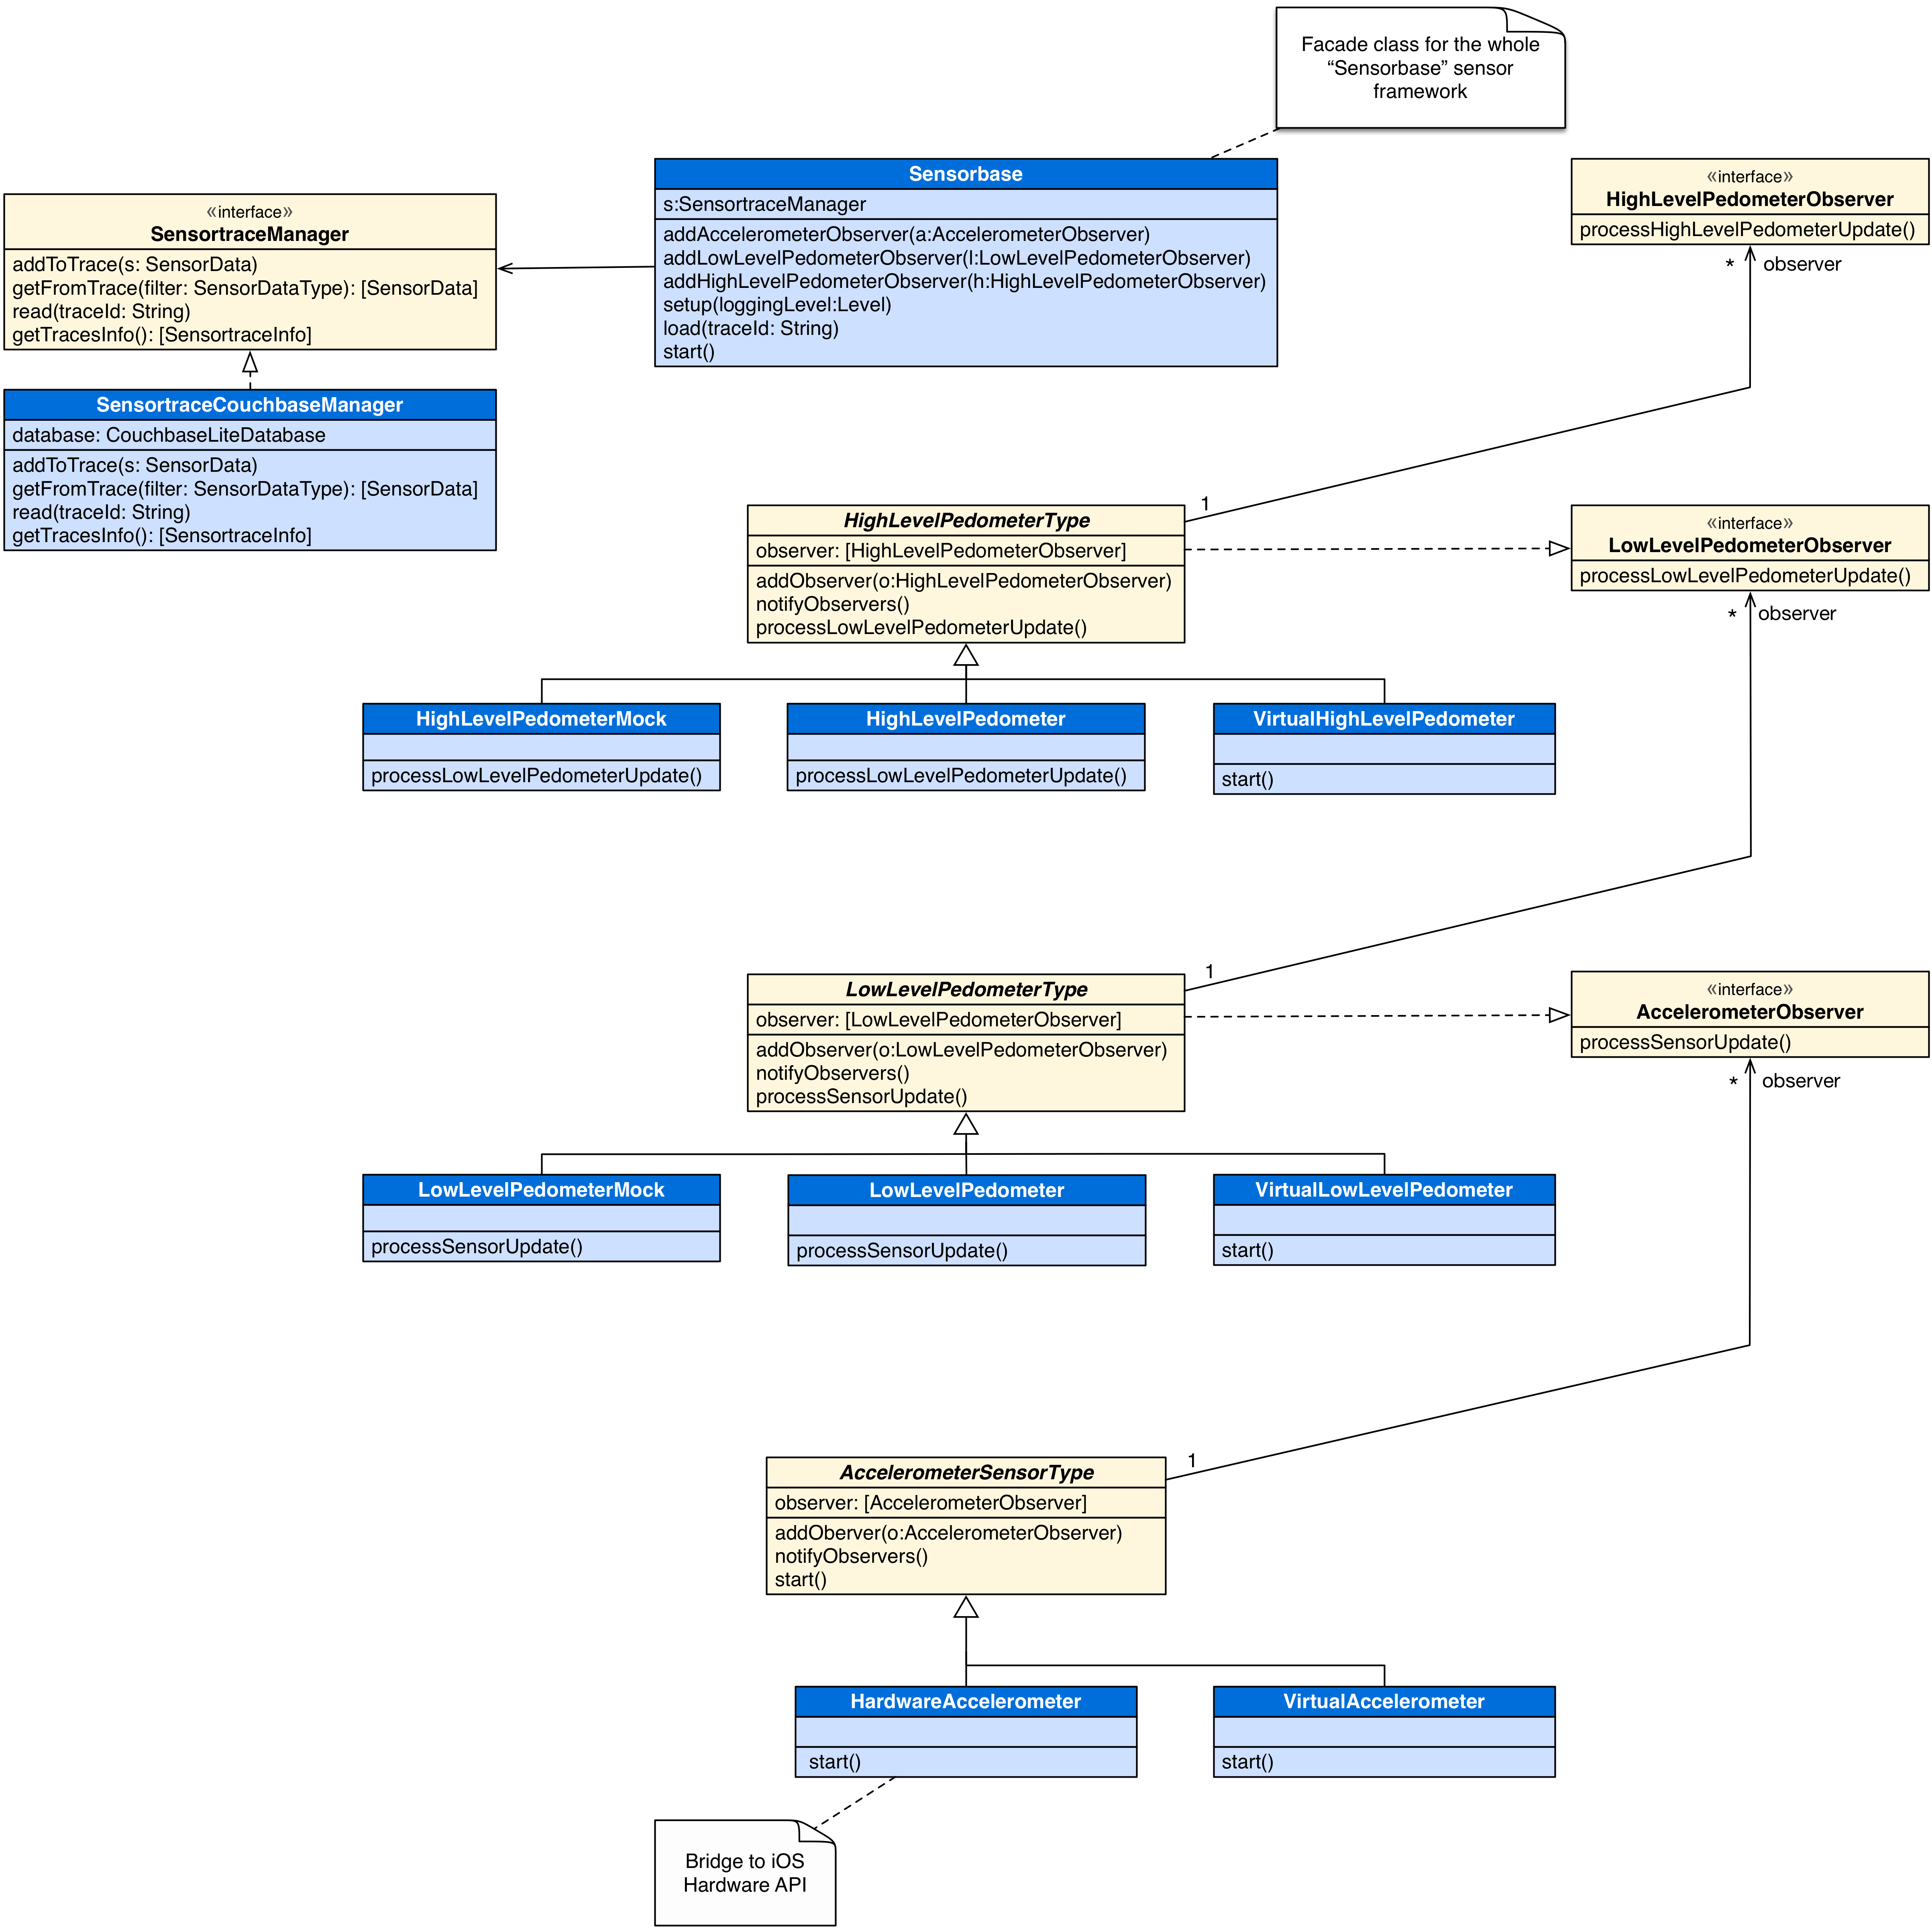
\includegraphics[width=1.0\textwidth]{class-diagram-guide-app.png}
\caption{Simplified Class Diagram for Sensor Data Processing}
\end{figure}

Mock: useful for Testing the underlying layer,
Adapter


\section{Sensors Layers}

Sensor data is saved to couchbase database.
Later access for replay (development), testing and presentations.
The backend can access this saved data for later analysis.

\section{Application Logic}

If not walking fast load and play current content.

If display is on show actions that user has to opt in, if display is off play automatically. 

\section{Presentation Layer}

Mockups
XCode Storyboard
Final App Screenshots